\documentclass[aspectratio=169]{beamer}
%\usetheme{Marburg}
\usepackage[utf8]{inputenc}
\usepackage[russian]{babel}
\usepackage[OT1]{fontenc}
\usepackage{amsmath}
\usepackage{amsfonts}
\usepackage{amssymb}
\usepackage{graphicx}
\usepackage{mathtools}
\usepackage{xcolor}
\usepackage{empheq}
\usepackage[many]{tcolorbox}
\usepackage{multirow}

\author{Николай Анохин}

\title{Задача и алгоритмы кластеризации}
%\setbeamercovered{transparent} 
\setbeamertemplate{navigation symbols}{} 
%\logo{} 
%\institute{} 
\date{} 
%\subject{}

\tcbset{highlight math style={enhanced,colframe=red,colback=white,arc=4pt,boxrule=1pt}}

\setbeamertemplate{caption}{\raggedright\insertcaption\par}

\begin{document}

\begin{frame}
\titlepage
\end{frame}

\begin{frame}{Обучение без учителя}

В задачах {\bf без учителя} значение целевой функции для объектов из обучающей выборки неизвестно. Решение таких задач подразумевает исследование ``скрытой структуры'' данных.

\vspace{2em}
Задача {\bf кластеризации} -- задача без учителя, подразумевающая разбиение множества объектов на непересекающиеся подмножества (кластеры).

\end{frame}

\begin{frame}{Мотивация}

\only<1>{Кластеризация позволяет больше узнать о данных}
\only<2>{Работать с кластерами удобнее, чем c отдельными объектами}
\only<3>{Кластеры можно использовать как признаки в других задачах}

\only<1>{
\begin{figure}
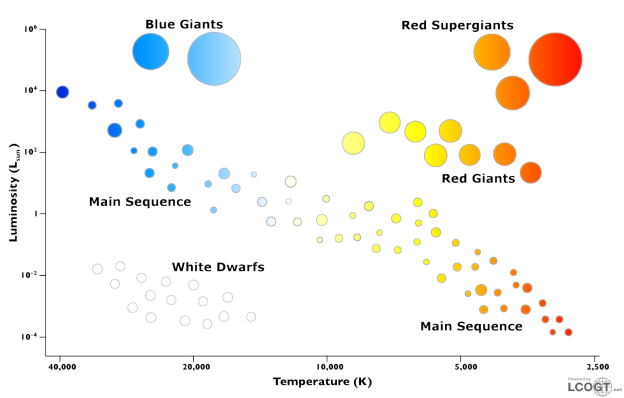
\includegraphics[height=0.6\textheight]{images/hrdiagram.png}
\caption{Диаграмма Герцшпрунга — Рассела\footnote{\url{https://lcogt.net/spacebook/h-r-diagram/}}}
\end{figure}
}

\end{frame}

\begin{frame}{Задача кластеризации}

\vspace{1em}
{\bf Дано.} Признаковые описания $N$ объектов $\mathbf{x} = (x_1, \ldots, x_m) \in \mathcal{X}$, образующие тренировочный набор данных $X$

\vspace{1em}
{\bf Найти.} Модель из семейства параметрических функций 
\[
H = \{h(\mathbf{x, \mathbf{\theta}}): \mathcal{X} \times \Theta \rightarrow \mathcal{Y} \mid \mathcal{Y} = \{1, \ldots, K\}\},
\]
ставящую в соответствие произвольному $\mathbf{x} \in \mathcal{X}$ один из $K$ кластеров так, чтобы объекты внутри одного кластера были похожи, а объекты из разных кластеров различались

\end{frame}


\end{document}